\documentclass[twoside,a4paper,12pt,openany]{book}

\usepackage[utf8]{inputenc}
\usepackage[spanish]{babel}
\usepackage{geometry}
\usepackage{makeidx}
\usepackage{graphicx}
\usepackage{subfigure}
\usepackage{subfig}
%\usepackage[Bjornstrup]{fncychap}
\usepackage{a4wide}
\usepackage{named}
\usepackage[table]{xcolor}
\usepackage{listings}
\usepackage{pdfpages}
\usepackage{appendix}
\usepackage{amsmath}
\usepackage{amsfonts}

% From texlive-science
\usepackage{algorithm}
\usepackage{algorithmic}

%\DeclareGraphicsExtensions{.jpg,.pdf,.png,.ps}

\usepackage{color}
\definecolor{gray97}{gray}{.97}
\definecolor{gray75}{gray}{.75}
\definecolor{gray45}{gray}{.45}

\pagestyle{headings}
\geometry{a4paper, left=3.5cm, right=2cm, top=3cm, bottom=2cm, headsep=1.5cm}

\widowpenalty=10000
\clubpenalty=10000
\hyphenpenalty=10000
\tolerance=10000
%Para que no corte las palabras al final de la linea.

% Latex command para crear listas sin espacio entre
% un item y otro.
\newenvironment{packed_item}{
\begin{itemize}
  \setlength{\itemsep}{1pt}
  \setlength{\parskip}{0pt}
  \setlength{\parsep}{0pt}
}{\end{itemize}}

% Latex command para crear listas umeradas sin 
% espacio entre un item y otro.
\newenvironment{packed_enum}{
\begin{enumerate}
  \setlength{\itemsep}{1pt}
  \setlength{\parskip}{0pt}
  \setlength{\parsep}{0pt}
}{\end{enumerate}}

% Configuracion del entorno lstlistings

\definecolor{dkgreen}{rgb}{0,0.6,0}
\definecolor{gray}{rgb}{0.5,0.5,0.5}
\definecolor{mauve}{rgb}{0.58,0,0.82}

\lstset{frame=tb,
  language=C++,
  aboveskip=3mm,
  belowskip=3mm,
  showstringspaces=false,
  columns=flexible,
  basicstyle={\small\ttfamily},
  numbers=none,
  numberstyle=\tiny\color{gray},
  keywordstyle=\color{blue},
  commentstyle=\color{dkgreen},
  stringstyle=\color{mauve},
  breaklines=true,
  breakatwhitespace=true,
  tabsize=3
}

% minimizar fragmentado de listados
\lstnewenvironment{listing}[1][]
{\lstset{#1}\pagebreak[0]}{\pagebreak[0]}

\lstdefinestyle{consola}
{basicstyle=\scriptsize\bf\ttfamily,
backgroundcolor=\color{gray75},
}

\lstdefinestyle{C}
{language=C,
}

\lstdefinestyle{yaml}
{language=yaml,
}

\makeindex

\begin{document}

\thispagestyle{empty}

\baselineskip 1.35\baselineskip

\vspace{2cm}

\begin{figure}[htb]
  \centerline{\resizebox{.60\textwidth}{!}{
\includegraphics{img/logo_urjc}}}
\end{figure}

\begin{center}
  {\Large {\bf Grado en Ingeniería en Telemática}}
  \vspace{5mm}
 
  {\large {Escuela Técnica Superior de Ingeniería Telecomunicación}}
  \vspace{5mm}

  {\large {Curso académico 2016/2017}}

  \vspace{1cm}

  {\large {\bf Trabajo Fin de Grado}}

  \vspace{2cm}

  {\Large {Navegación para robots móviles en entornos domésticos\\[1cm] }}

  \vspace{5cm}
  {\bf Autor}: Jonathan Ginés Clavero
  {\bf Tutor}: Francisco Martín Rico 
\end{center}

\clearpage
\newpage{\pagestyle{empty}\cleardoublepage}
\thispagestyle{empty}

\vspace{5cm}
\makebox[15cm][r]{
  \begin{tabular}{ll}
  \emph{A}
  \end{tabular} 
}

\clearpage
\newpage{\pagestyle{empty}\cleardoublepage}
\thispagestyle{empty}

\vspace{5cm}
\textbf{\huge{Agradecimientos}}\\

\clearpage
\newpage{\pagestyle{empty}\cleardoublepage}

%%%%%%%%%% RESUMEN %%%%%%%%
\newpage{\pagestyle{empty}\cleardoublepage} 
\vspace{5 cm}
\textbf{\Huge{Resumen}}
\vspace{1.5 cm}



                                %\pagenumbering{roman}

                                %\setcounter{page}{1}
\frontmatter
\tableofcontents

\listoffigures
                                %\setcounter{page}{1}
                                %\pagenumbering{arabic}
%\listoftables

\mainmatter

% Init counter page
\setcounter{page}{1}

% Capitulo 1
\chapter{Introducción}
\label{cap:introduccion}

\section{Robótica móvil}
\label{cap:roboticamovil}
Los robots móviles son máquinas con la capacidad de desplazarse por un entorno. Para ello hacen uso de un sistema de automoción, ya sean ruedas, patas u orugas. 
La robótica móvil está sufriendo un gran crecimiento debido al abaratamiento del hardware y las grandes oportunidades que nos ofrecen, tanto en materia de educación como en materia industrial. 
Cuando nos encontramos con un problema en el que un robot móvil puede ser la mejor solución tendremos que tener en cuenta los siguientes problemas a solucionar:
\begin{itemize}
\item \textbf{Percepción} Para resolver este problema equiparemos a nuestro robot de sensores, como puede ser una cámara, un láser, sensores de odometría o bumpers para obtener información acerca de qué hay en el escenario en el que se encuentra el robot.
\item \textbf{Localización} Una vez resuelto el problema de conocer que hay cerca del robot, necesitamos conocer la posición del robot dentro del escenario. Esto se puede resolver con algoritmos como MonteCarlo, con cámaras cenitales, triangulación con balizas, etc. Para resolver la localización también es común el uso de mapas. 
\item \textbf{Navegación} La característica principal de los robots móviles es que tienen la capacidad de desplazarse, pero la navegación no solo se cumple cuando el robot se mueve, el robot debe moverse a un punto determinado, de una forma segura, es decir sin chocar con los objetos del escenario, y de la forma más eficaz posible. Dentro de la navegación se pueden distinguir 2 partes, la navegación local que se ocupa del movimiento del robot y de evitar obstáculos y la navegación global qué establece rutas.
\item \textbf{Inteligencia} El siguiente problema se encuentra en un nivel de abstracción más alto. El problema de la inteligencia se refiere a qué tiene que hacer el robot, qué finalidad debe cumplir.
\item \textbf{Autonomía} Habrá momentos en los que el robot deberá tomar algunas decisiones, en referencia a su estado en el escenario, por ejemplo si se acerca mucho a una pared, o si llega a su destino correctamente.
\item \textbf{Interacción con los humanos} Los robots suelen crearse para facilitarnos una tarea o asistirnos en nuestro día a día, por esto los robots deben contar con una interfaz hombre-maquina con la que comunicarnos cosas o con la que nosotros podamos ayudar al robot para así mejorar sus acciones.
\end{itemize}

\section{Mapeado}
\label{cap:mapeado}
Crear un mapa de un escenario puede sernos realmente útil ya que servirán al robot como fuente de información para resolver problemas de Localización y de Navegación. Estos mapas pueden ser creados por un humano, midiendo las paredes y los objetos de un escenario para más tarde transformarlo en una imagen que el robot pueda leer, o puede ser creado directamente con un robot móvil. Esta segunda opción nos permite realizar mapas de zonas que pueden resultar inaccesibles para el ser humano, como puede ser una zona radioactiva u otro planeta del sistema solar.

\begin{figure}[hbtp]
  \begin{center}
    \subfigure[Mapa láser]{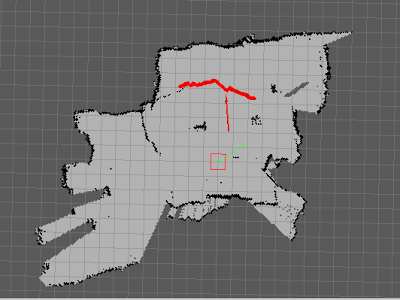
\includegraphics[width=6cm,height=5cm]{img/cap1/mapa1}}
    \subfigure[Mapa RGBD]{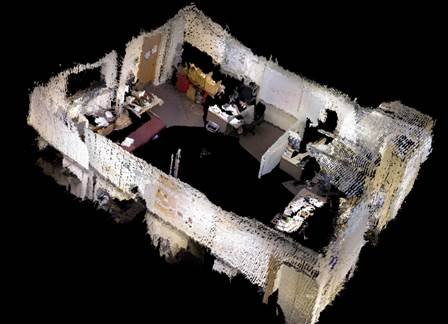
\includegraphics[width=6cm,height=5cm]{img/cap1/mapa2}}
  \end{center}
  \caption{Ejemplos de mapas}
  \label{fig:maps-ej}
\end{figure}
Para llevar a cabo el mapeo de un escenario con un robot móvil deberemos equipar a nuestro robot con sensores capaces de medir distancias, tales como una cámara RGBD o un láser. La cámara RGBD nos proporciona una nube de puntos en 3D, por lo que nos proporciona una información muy rica del entorno pero el tratamiento de esta información resulta muy costoso. El láser nos proporciona un array de distancias en 270º, estas distancias suelen ser muy precisas y su tratamiento es muy liviano, aunque solo contamos con el plano en el que se ubica el láser. 

En ese trabajo se expondrá una nueva opción de mapeado que resultará de la mezcla de las dos opciones vistas anteriormente. Partiremos de un mapa creado por nosotros de un escenario y el robot irá añadiendo dinámicamente los objetos que vaya encontrando y no estén representados en este mapa inicial. Esta nueva visión nos ha proporcionado muy buenos resultados, tanto que fue integrada como algoritmo de navegación en el robot del equipo GentleBots, del cual formamos parte, y con el que participamos en la Robocup 2016 de Leipzig, en la categoría RoboCup@Home.

\section{RoboCup@Home}
\label{cap:robocup}
La categoría RoboCup@Home tiene como objetivo desarrollar la tecnología de robots de servicio y asistencia para futuras aplicaciones domésticas. Es el mayor concurso anual internacional de robots de servicio autónomos y es parte de la Robocup.

\begin{figure} [hbtp]
  \begin{center}
    
\includegraphics[width=5cm]{img/cap1/logoRobocupHome}
  \end{center}
  \caption{Robocup@Home.}
  \label{fig:logoRobocupHome}
\end{figure}

Se utiliza un conjunto de pruebas de referencia  para evaluar las capacidades y el rendimiento de los robots en un entorno del hogar no estandarizado. La atención se centra en los siguientes dominios, pero no se limita exclusivamente a ellos:

\begin{itemize}
\item \textbf{Interacción y cooperación robot-humano} 
\item \textbf{Navegación y cartografía en entornos dinámicos} 
\item \textbf{Visión artificial y reconocimiento de objetos en condiciones de luz natural} 
\item \textbf{Manipulación de objetos} 
\item \textbf{Comportamientos adaptativos} 
\item \textbf{Integración de comportamientos}
\item \textbf{Inteligencia ambiental}  
\item \textbf{Normalización e integración de Sistemas}  
\end{itemize}

Cada año el escenario en el que se realizan las pruebas se actualiza para parecerse cada vez más a un escenario real de un ambiente doméstico. En los primeros años solo constaba de una salón y una cocina pero cada vez se incorporan más estancias, como pasillos, habitaciones o zonas de jardín. Los escenarios del año 2016 constaban de cocina, sala de estar, habitación, pasillo y entrada. Además cada escenario tenia 3 puertas para salir al exterior.

RoboCup@Home acaba con las finales, donde los 5 equipos con las puntuaciones más altas pueden realizar la prueba final. Los equipos son calificados por un jurado formado por especialistas y no especialistas en robótica, como puede ser empresarios, especialistas en interacción hombre-máquina, personas de diseño industrial, el público o la prensa. En las finales se enfatiza menos en las cuestiones técnicas, ya que si se llega a la final significa que los equipos son muy buenos en el plano técnico.

\section{Estructura de la memoria}
\label{cap:estructuradelamemoria}
En este documento se describen los aspectos más relevantes del desarrollo del algoritmo. La memoria está dividida en ocho capítulos. En este primer capítulo se ha presentado el contexto en el que se va a desarrollar el proyecto. En el segundo capítulo se define el problema concreto y se establecen los requisitos y los objetivos del proyecto. En el tercer capítulo se exponen y describen el robot con el que se ha trabajado y las distintas herramientas que hemos utilizado o mejorado. El montaje del robot y el diseño de conectividad seguido se explica en el capítulo cuatro. En el capítulo cinco se expone el algoritmo de mapping creado. El sexto capítulo expondrá la navegación semántica desarrollada y como usa el algoritmo de mapping. En el séptimo capítulo expondremos los experimentos llevados a cabo y un pequeño diario de nuestra experiencia en la Robocup. Por último en el octavo capítulo se expondrán las conclusiones del trabajo.


% Capitulo 2
\chapter{Objetivos y Metodología}
\label{cap:objetivos}

%Una vez presentado el contexto en el que se sitúa este proyecto, en este capítulo se fijan los objetivos y requisitos que debe seguir la solución. Para ello primero se describirá el problema y se explicará porqué es importante hacer el seguimiento de los objetos; a continuación se fijarán los objetivos y requisitos en función del problema y, por último, se expondrá la metodología seguida.

\section{Descripción del problema y requisitos}
\label{sec:descripciondelproblema}

La navegación en entornos dinámicos, como puede ser una casa o una institución pública, supone un gran reto que superar ya que las personas o las mascotas pueden acercarse o cruzarse delante del robot o podríamos encontrarnos objetos del mobiliario que han sido movidos de su posición original y se encuentran en nuestro camino. En este escenario el robot no debería nunca ni chocar ni perderse en el entorno y debe llegar al destino impuesto por la mejor ruta disponible.\\

Por ejemplo, si nuestro robot está yendo desde el salón a la cocina de nuestra casa pero en su camino habitual y más optimo se encuentra un mueble, el robot debe darse cuenta rápidamente, esquivarlo, proseguir con su camino y ademas recordarlo para que cuando volvamos al salón de vuelta podamos esquivarlo más fácilmente.Por otro lado en nuestra casa también habrá personas, estas personas se moverán casi constantemente por la estancia por lo que no será del todo correcto tenerlas en cuenta a la hora de planificar nuestra ruta para navegar de un sitio a otro de la casa pero si que será muy importante no chocar con ellas.\\

Para analizar el entorno del robot usaremos el sensor láser, este sensor destaca por su alta precisión y su corto tiempo de procesado.\\

%\begin{figure}[hbtp]
%  \centering
%  \subfloat[Cálculo de la trayectoria de la bola]{
%    \includegraphics[width=8.5cm]{img/cap2/goalie_following_ball}
%  }
%  \subfloat[Movimiento de parada]{
%    \includegraphics[width=6.4cm]{img/cap2/goalie_jump}
%  }
%  \caption{Portero intentando parar un disparo a puerta}
%  \label{fig:portero_trayectoria_bola}
%\end{figure}

%El sistema debe cumplir los siguientes requisitos:
%\begin{enumerate}
%\item \textbf{Posición y velocidad.} El sistema que se implemente deberá estimar la posición y velocidad de los objetos. Estas medidas deberán ir acompañadas de una incertidumbre que indique su fiabilidad.
%\item \textbf{Escalable.} Se debe poder seguir varios objetos al mismo tiempo, incluso si se trata de objetos homogéneos indistinguibles para el detector.
%\item \textbf{Tiempo real.} El algoritmo se ejecuta en tiempo real. Éste debe ser lo suficientemente eficiente como para poder ser ejecutado en un robot sin perjudicar al resto de las funcionalidades, y debe ser ligero computacionalmente.
%\item \textbf{General.} El algoritmo debe poder ser utilizado con cualquier tipo de detector que devuelva como mínimo la posición de un objeto en un instante determinado del tiempo.
%\item \textbf{Varias instancias.} Se podrán ejecutar varias instancias del algoritmo paralelamente. Cada una de las instancias debe ser independiente de la otra, ya que pueden ejecutarse a frecuencias distintas.
%\item \textbf{Objetos dinámicos vs estáticos.} La naturaleza de los objetos puede variar y ser tanto dinámica como estática. El algoritmo debe ser capaz de adaptarse a ambas situaciones.
%\item \textbf{Extensible.} Se diseñará el algoritmo de tal forma que sea fácil ampliar su funcionalidad.
%\item \textbf{Independiente de la plataforma.} Es importante que el núcleo del algoritmo sea independiente de la plataforma en la que se pruebe para facilitar su exportación a otras plataformas.
%\item \textbf{Precisión y Robustez.} El algoritmo debe mejorar la precisión y robustez de los datos proporcionados por el detector.
%\end{enumerate}

\section{Objetivo del proyecto}
\label{sec:objetivos}

Se quiere diseñar un algoritmo genere un mapa en tiempo real, el cual será usado por el nodo de navegación de ROS para navegar por un entorno doméstico, ya sea indicando una posición x,y en el mapa o indicándole una estancia a la que navegar. Este mapa se construirá a partir de la mezcla de 3 mapas, mapa estático, mapa de largo plazo y mapa de corto plazo.\\
%hablar del mapa semántico
En primera instancia el algoritmo se validará haciendo uso de un simulador en el que se representa una casa con varios tipos de muebles, ya que resulta más fácil de depurar un algoritmo en un entorno virtual, que en un entorno real. Posteriormente el algoritmo se probará en distintas recreaciones de escenarios reales ,y se harán las modificaciones oportunas para adaptarlo al entorno real, y por ultimo se llevará a la competición.\\

Para simplificar la resolución del problema se ha dividido el proyecto en varios subobjetivos:

\begin{enumerate}
\item Se usarán las herramientas por defecto que nos ofrece ROS para creare el mapa de corto plazo en referencia a las mediciones tomadas por el laser. En un primer paso solo añadiremos los diferentes objetos que percibamos.
\item Se ampliará el algoritmo anterior para poder añadir y eliminar objetos que aparezcan o desparezcan del entorno. 
\item Se desarrollará un algoritmo para mezclar los mapas entre sí y así generar tanto el mapa de largo plazo como el mapa que usaremos para la navegación.
\item Se creará un servidor de mapas dinámicos que se inicializará con los mapas estático y de largo plazo y que generará el mapa final mezclando de loa mapas de largo plazo y de corto plazo.
\item Se usará el mapa final como parámetro del paquete de navegación de ROS, \textit{move base}, y del paquete de localización de ROS \textit{amcl}.
\item se generará y usará un mapa semántico, en el que cada nivel de gris se asocie con una etiqueta para después ordenar al robot que navegue a dichas etiquetas.
\end{enumerate}

\section{Metodología de desarrollo}
\label{sec:metodologiadedesarrollo}

En el desarrollo del sistema descrito, el modelo de ciclo de vida utilizado ha sido el modelo en espiral basado en prototipos. Este modelo permite desarrollar el proyecto de forma incremental, aumentando la complejidad progresivamente y haciendo posible la generación de prototipos funcionales. Este planteamiento permite obtener productos parciales al final de cada ciclo que pueden ser evaluados, ya sea total o parcialmente. Esto facilita la adaptación a los cambios en los requisitos, circunstancia muy común en los proyectos de investigación.\\

\begin{figure} [hbtp]
  \begin{center}
    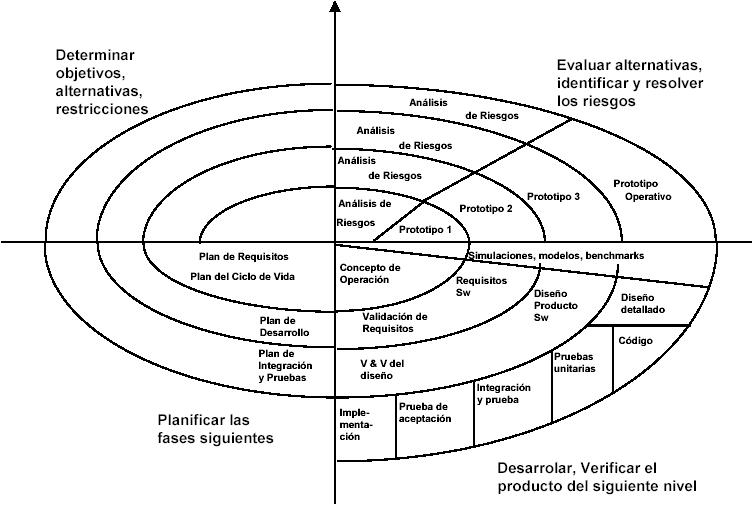
\includegraphics[width=16cm]{img/cap2/modelo_espiral}
  \end{center}
  \caption{Modelo en espiral.}
  \label{fig:modelo_espiral}
\end{figure}\

El ciclo de vida de este modelo está dividido en ciclos. Cada ciclo representa una fase del proyecto y está dividido, a su vez, en 4 partes. Cada una de las partes tiene un objetivo distinto:

\begin{itemize}
\item \textbf{Determinar objetivos.} Se establecen las necesidades que debe cumplir el sistema en cada iteración teniendo en cuenta los objetivos finales. Según avanzan las iteraciones aumenta el coste del ciclo y su complejidad.
\item \textbf{Evaluar alternativas.} Se determinan diferentes formas de alcanzar los objetivos que se han establecido en la fase anterior. Se aborda el problema desde distintos puntos de vista, como, por ejemplo, el rendimiento del algoritmo en tiempo y espacio. Además, se consideran explícitamente los riesgos, intentando mitigarlos al máximo.
\item \textbf{Desarrollar y verificar.} Se desarrolla el producto siguiendo la mejor alternativa para poder alcanzar los objetivos del ciclo. Una vez diseñado e implementado el producto, se realizan las pruebas necesarias para comprobar su funcionamiento.
\item \textbf{Planificar.} Teniendo en cuenta los resultados de las pruebas realizadas, se planifica la siguiente iteración, se revisan los errores cometidos y se comienza un nuevo ciclo de la espiral.
\end{itemize}

\section{Plan de trabajo}
\label{sec:plandetrabajo}

Para poder abordar el problema se han marcado una serie de subobjetivos ha completar. Dichos hitos son los siguientes:

\begin{enumerate}
\item Estudio y comprensión de la composición de un mapa y como construirlo. Nos apoyaremos en las herramienta ofrecidas por ROS y que resultaran básicas para este fin, dicha herramientas son \textit{TF} \footnote{http://wiki.ros.org/tf} y \textit{Costmap}\footnotemark .
\footnotetext{http://wiki.ros.org/costmap\_2D}
\item Primer subobjetivo. Una vez conocido como funcionan los \textit{costmap} procederemos a crear un pequeño nodo en el que se cree un mapa con las observaciones instantáneas que percibimos con el láser.
\item Segundo subobjetivo. Extender el algoritmo anterior para poder añadir y eliminar objetos según entren o salgan de la escena.
\item Tercer subobjetivo. Modificar el paquete \textit{map\_server} para que acepte varios mapas como entrada y estudiar la manera de mezclar los mapas entre sí.
\item Fase de pruebas. Se le pasará al paquete de navegación de ROS, \textit{move\_base} ,el mapa resultante y se harán pruebas de navegación en el simulador y en el robot real.
\item Cuarto subobjetivo. Crear el mapa semántico, especificando las etiquetas naturales que tendrá una casa, salón, cocina, habitación... y usarlo para poder ir a la estancia que le indiquemos.

\end{enumerate}


% Capitulo 3
\chapter{Entorno y herramientas}
\label{cap:entorno}

\section{Robot Kobuki}
\label{cap:robot}
\section{ROS}
\label{cap:ros}
\section{Software en ROS para el mapeado, localización y navegación}
\label{cap:softwarederos}

\subsection{Costmap\_2D}
\label{sec:costmap2d}
Un \textit{costmap} es una estructura de datos ofrecida por ROS y compuesta por un grid de ocupación y los metadatos de este grid. Cada celda del grid toma valores entre 0 y 255, donde 0 corresponde a una celda vacía, los valores entre 1 y 254 representan la probabilidad de que una celda está ocupada y el valor 255 se reserva para el desconocimiento. Cada valor se asocia con un nivel de gris, como se puede ver en la imagen.
\begin{figure} [hbtp]
  \begin{center}
    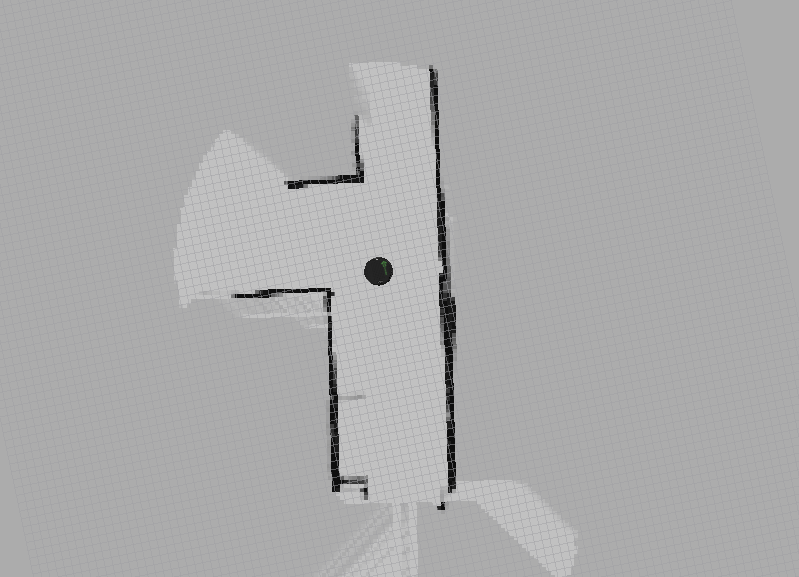
\includegraphics[width=7.5cm]{img/cap4/costmap-ejemplo}
  \end{center}
  \caption{Ejemplo visual de un costmap.}
  \label{fig:costmap-ejemplo}
\end{figure}\

Para poder representar la ocupación de un objeto en un \textit{costmap} es necesario hacer uso de las transformadas entre frames que nos ofrece ROS.

\subsubsection{tf}
\label{subsubsec:tf}
Cualquier robot está compuesto por multitud de piezas móviles, como puede ser la propia base del robot o la pinza de un brazo robótico. Cada una de estas piezas se pueden representar con un \textit{frame}. Ademas existen también otros \textit{frames} que pueden interesarnos, como puede ser el \textit{frame} de world o el \textit{frame} de map.
\begin{figure} [hbtp]
  \begin{center}
    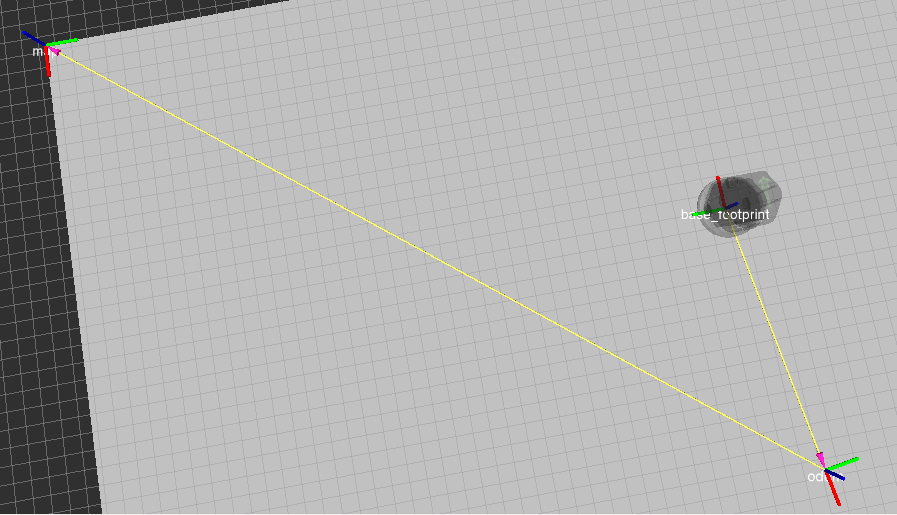
\includegraphics[width=12cm]{img/cap4/frames}
  \end{center}
  \caption{A la izquierda el frame map y a la derecha los frames de odom y base\_footprint}
  \label{fig:frames}
\end{figure}

Usamos las \textit{tf} para poder representar información relativa a uno de estos frames. Esto puede sernos de utilidad, por ejemplo, si queremos conocer la posición de un objeto que hemos cogido con nuestra pinza respecto a la base de nuestro robot, o cual es la posición relativa de un objeto que estamos percibiendo con el láser respecto a nosotros o respecto al mapa.

Cuando trabajamos con mapas es importante que todo lo que se representa en él sea respecto al frame map. De este modo nuestro mapa puede ser usado por otros nodos, como el nodo de navegación, o en cualquier otro escenario. \pagebreak


\subsection{AMCL}
\label{sec:amcl}
\textit{AMCL}\footnote{http://wiki.ros.org/amcl} es un paquete de localización que implementa un algoritmo de Monte Carlo, el cual usa un filtro de partículas para localizar al robot sobre un mapa que previamente le proporcionamos.
\subsubsection{Filtro de partículas}
El algoritmo del filtro de partículas se divide en 4 etapas: Inicialización, actualización, estimación y predicción. 
En la etapa de inicialización se ``lanzan'' una serie de partículas cercanas a la posición inicial del robot. Estas partículas ademas de una posición en el espacio también tendrán una dirección. Podemos ver un ejemplo gráfico en la imagen \ref{fig:initamcl}

\begin{figure}[hbtp]
  \begin{center}
    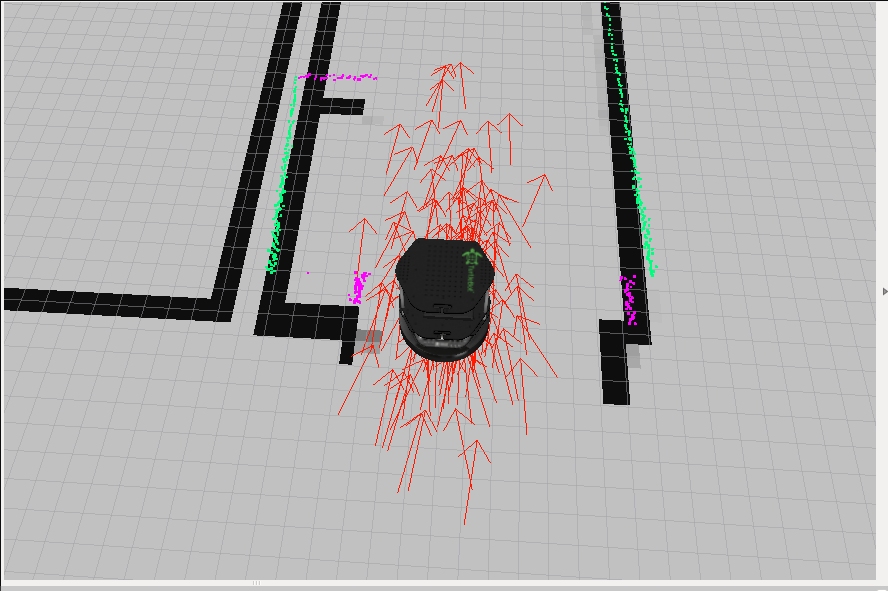
\includegraphics[width=10cm,height=7cm]{img/cap3/initamcl}
  \end{center}
  \caption{Inicialización del filtro de partículas}
  \label{fig:initamcl}
\end{figure}
Vemos como se han generado muchas partículas alrededor del robot y que cada una tiene una dirección más o menos acertada con la dirección del robot.

En este punto del algoritmo se compara la percepción del láser del robot en el punto en el que se encuentra con la percepción que tendría si tuviera la posición y la dirección de cada una de las partículas que generamos. Cuanto más acertada sea la suposición anterior, más valor se le da a esa partícula. Así nos encontraremos que las partículas que están más cercanas a la posición del robot cobran más valor y las que están más lejos y con una dirección totalmente errónea tienen menos valor. Esta fase es la llamada de Actualización. 

En la siguiente fase, llamada de Estimación, nos quedamos con las partículas que más valor tenían para volver a lanzarlas en la siguiente fase del algoritmo.

En la ultima fase, fase de Predicción, lanzamos las partículas de nuevo con el valor que tenían y su posición, añadiéndole un pequeño ruido.
En este punto del algoritmo también se corrige la posición del robot a la posición de la partícula con más valor.
Una vez completado el algoritmo se vuelve a la fase de Actualización y se repite hasta que el robot esté perfectamente localizado en el 
mapa.

\begin{figure}[hbtp]
  \begin{center}
    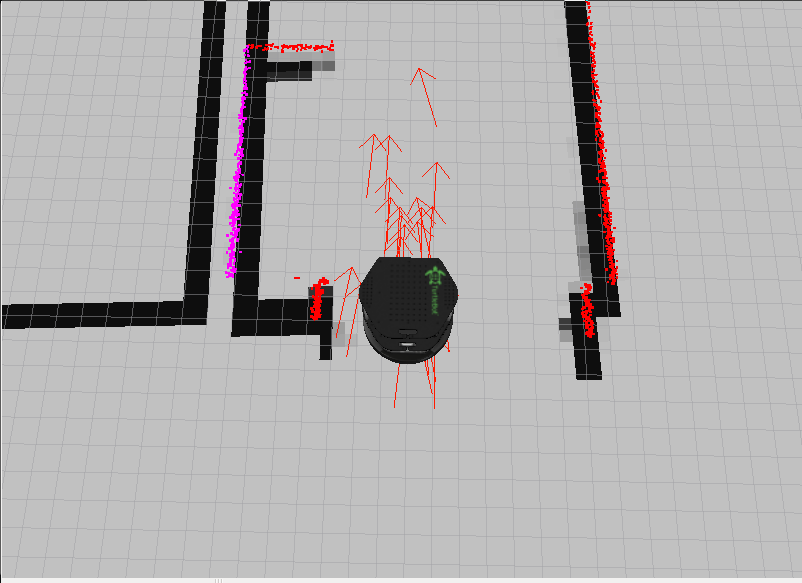
\includegraphics[width=10cm,height=7cm]{img/cap3/actamcl}
  \end{center}
  \caption{El robot se vá acercando a la posición ideal}
  \label{fig:actamcl}
\end{figure}
\pagebreak

Observamos como la linea color de la parte derecha de la imagen \ref{fig:actamcl}, correspondiente a las muestras tomadas con el láser, está más cerca de la linea del mapa que en la imagen \ref{fig:initamcl} que se aprecia que no está alineada. Esto es fruto de la corrección que se va haciendo de la posición. También observamos que hay menos partículas, esto es fruto de la convergencia hacia la posición correcta.

\begin{figure}[hbtp]
  \begin{center}
    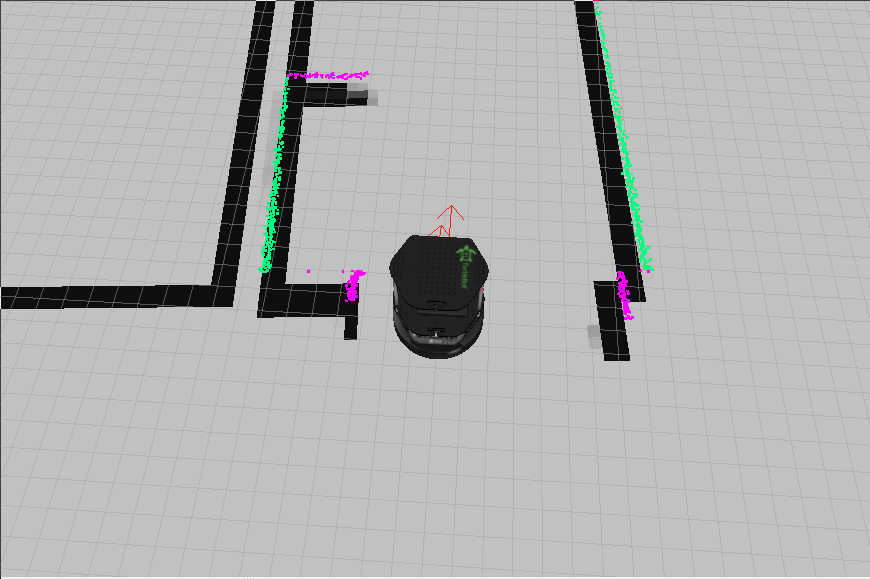
\includegraphics[width=10cm,height=7cm]{img/cap3/finamcl}
  \end{center}
  \caption{El robot se encuentra totalmente localizado}
  \label{fig:finamcl}
\end{figure}

En la imagen \ref{fig:finamcl} vemos como el número de partículas se ha reducido mucho, ya que se ha llegado a casi una estimación de la posición del robot muy cerca de la posición real. Vemos también que las lineas de color correspondientes a las muestras del láser están alineadas con el mapa.

Para el uso del paquete \textit{amcl} en nuestro algoritmo fue necesaria la realización de una pequeña modificación. Esta modificación se refiere a que el paquete por defecto solo usa un mapa y lo obtiene al principio de la ejecución del algoritmo. Si le llegaba un nuevo mapa reiniciaba por completo el algoritmo. Esto nos generaba un problema, ya que en el algoritmo propuesto se publica un mapa por cada iteración y el paquete por defecto se reiniciaba constantemente. El efecto que producía es que el robot siempre se encontraba en la posición inicial y aunque lo moviéramos siempre ocupaba la misma posición en el mapa. En nuestro \textit{amcl} modificado se usa el mapa que se obtiene en cada iteración y sobre el se calcula la posición del robot, sin reiniciar en ningún momento el algoritmo.

\subsection{Navigation}
\label{sec:navigation}
\textit{Navigation}\footnote{http://wiki.ros.org/navigation} es un paquete de ROS que toma información de la odometria, los sensores y la posición inicial y la posición a 

% Capitulo 4
\chapter{Servidor de mapas dinámico}
\label{cap:sevidordemapasdinamico}


En este capítulo se explica la construcción y el funcionamiento del servidor de mapas dinámico. En primer lugar se explica que és, para que se utiliza y como se construye un \textit{costmap}. En segundo lugar se explica como se construyen los mapas que componen el algoritmo y por último se explica como se combinan estos mapas para generar el mapa usado en la navegación.

\section{Costmap\_2D}
\label{sec:costmap2d}
Un \textit{costmap} es una estructura de datos ofrecida por ROS y compuesta por un grid de ocupación y los metadatos de este grid. Cada celda del grid toma valores entre 0 y 255, donde 0 corresponde a una celda vacía, los valores entre 1 y 254 representan la probabilidad de que una celda está ocupada y el valor 255 se reserva para el desconocimiento. Cada valor se asocia con un nivel de gris, como se puede ver en la imagen.
\begin{figure} [hbtp]
  \begin{center}
    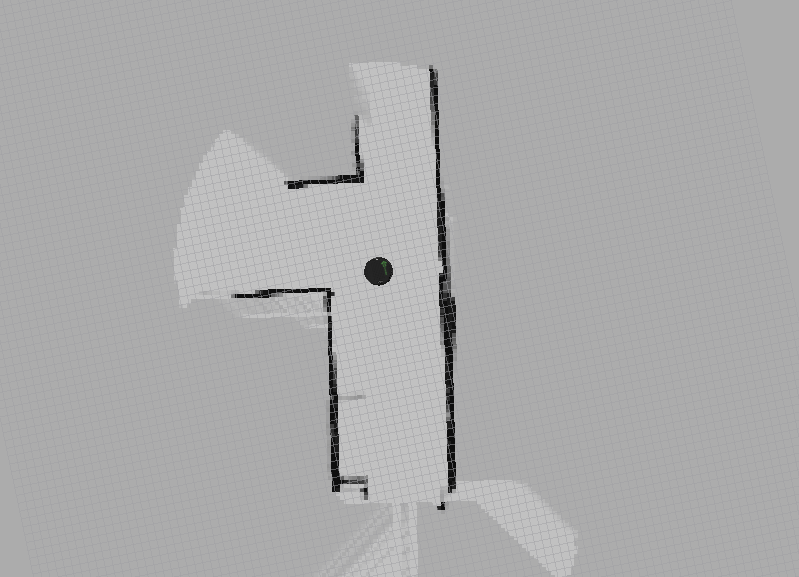
\includegraphics[width=7.5cm]{img/cap4/costmap-ejemplo}
  \end{center}
  \caption{Ejemplo visual de un costmap.}
  \label{fig:costmap-ejemplo}
\end{figure}\

Para poder representar la ocupación de un objeto en un \textit{costmap} es necesario hacer uso de las transformadas entre frames que nos ofrece ROS.

\subsubsection{tf}
\label{subsubsec:tf}
Cualquier robot está compuesto por multitud de piezas moviles, como puede ser la propia base del robot o la pinza de un brazo robótico. Cada una de estas piezas se pueden representar con un \textit{frame}. Ademas existen tambien otros \textit{frames} que pueden interesarnos, como puede ser el \textit{frame} de world o el \textit{frame} de map.
\begin{figure} [hbtp]
  \begin{center}
    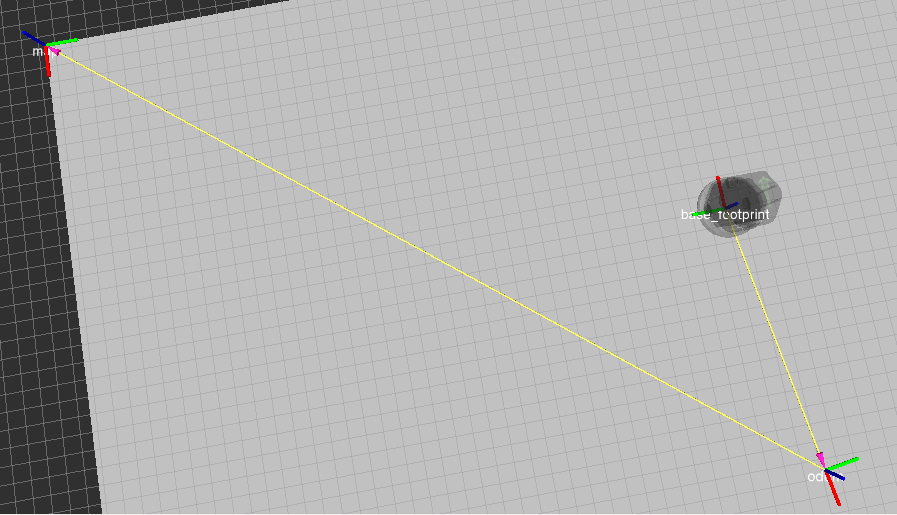
\includegraphics[width=12cm]{img/cap4/frames}
  \end{center}
  \caption{A la izquierda el frame map y a la derecha los frames de odom y base\_footprint}
  \label{fig:frames}
\end{figure}

Usamos las \textit{tf} para poder representar información relativa a uno de estos frames. Esto puede sernos de utilidad, por ejemplo, si queremos conocer la posición de un objeto que hemos cogido con nuestra pinza respecto a la base de nuestro robot, o cual es la posición relativa de un objeto que estamos percibiendo con el laser respecto a nosotros o respecto al mapa.

Cuando trabajamos con mapas es importante que todo lo que se representa en él sea respecto al frame map. De este modo nuestro mapa puede ser usado por otros nodos, como el nodo de navegación, o en cualquier otro escenario. \pagebreak

\section{Tipos de mapas}

En este apartado se describirá la metodologia seguida para la construcción de cada uno de los tres mapas usados por el algoritmo.

\subsection{Mapa estático}
El mapa estático se caracteriza por incluir las partes inmutables del escenario, como son las paredes o las puertas. La mejor manera de construirlo es medir todo el escenario y crear el mapa usando una herramienta de diseño gráfico. En este caso se ha usado \textit{Gimp}.
Este mapa nos servirá como base para crear el mapa de largo plazo.

\begin{figure} [hbtp]
  \begin{center}
    \includegraphics[width=7cm]{img/cap4/mapaestatico}
  \end{center}
  \caption{Mapa estático}
  \label{fig:mapaestatico}
\end{figure}

\subsection{Mapa de corto plazo}
El mapa de corto plazo se caracteriza por ser un mapa en el que se representa los objetos que el robot va percibiendo. Este mapa se inicializa con el valor 255, lo que indica una incertidumbre total. En el instante en el que el algoritmo de construcción del mapa comienza a iterar comenzarán a corregirse estos valores iniciales, asignando el valor 0 a las celdas que corresponden con zonas libres e incrementando desde 0 hasta 254 el valor de las celdas que se perciben como ocupadas. \\

{EJEMPLO CODIGO}\\

El algoritmo propuesto destaca por la capacidad de no solo añadir objetos al mapa, si no ademas eliminarlos si los objetos desaparecen del lugar que ocupaban. Para ello se compara cada muestra de datos con el mapa que estamos generando y si en dicha muestra existen celdas libres que en el mapa están ocupadas se decrementa el valor de dicha celda en el mapa. La cuantia del decremento se puede modelar, consiguiendo asi que el robot olvide más lentamente o más rapidamente los objetos que desaparecen del escenario.\\

{EJEMPLO CODIGO}\\
{EJEMPLO GRAFICO}\\

\subsection{Mapa de largo plazo}
El mapa de largo plazo se inicializa con los valores del mapa estático y se caracteriza por incluir los objetos que tienen un valor muy alto en el mapa de corto plazo, por tanto tenemos un mapa con objetos que han perdurado en el mapa a corto plazo durante un largo periodo de tiempo y que podemos considerar que son objetos estáticos del escenario. 
Este mapa tambien es dinámico, por lo que tambien elimina los objetos del mapa si estos desaparecen del escenario. Para ello se compara el mapa de largo plazo con el mapa de corto plazo. Si una celda en el mapa de largo plazo tiene un valor que indica que está ocupada y en el mapa de corto plazo esa misma celda tiene un valor que indica que está libre, siempre y cuando esa celda no pertenezca a una celda de una pared, se decrementa su valor en el mapa de largo plazo. La cuantia de este decremento tambien puede modelarse, regulando asi la memoria que tenemos de los objetos que hemos añadido a este mapa.\\

{EJEMPLO CODIGO}\\
{EJEMPLO GRAFICO}\\

Adicionalmente este mapa se guarda cada cierto tiempo en un fichero. Asi por ejemplo podemos tener un cuenta una mesa dentro del salón de una casa. Esto nos permitiria planificar una ruta para la navegación en la que podriamos esquivar esta mesa con facilidad y llegar a nuestro destino lo más rápido posible.



\section{Construcción del mapa final}
\label{sec:construccionmap}



% Capitulo 5
\chapter{Mapas dinámicos}
\label{cap:mapasdinamicos}
En este capítulo se expondrá el sistema creado para la composición de un mapa dinámico que pueda ser usado por paquetes de ROS como \textit{move\_base} o \textit{amcl} y que nos sirva para navegar por el ámbito doméstico de una forma más eficaz y segura de lo que lo haríamos usando un mapa estático o un sistema de \textit{SLAM}.

\section{Arquitectura del sistema}
\label{cap:arquitecturadelsistema}
El sistema propuesto pretende sustituir al nodo map\_server, ya que este nodo solo publica un mapa estático y esto presenta una serie de problemas que veremos más adelante, por tanto nos centramos en esa parte del modelo de navegación de ROS.
\begin{figure} [H]
  \begin{center}
    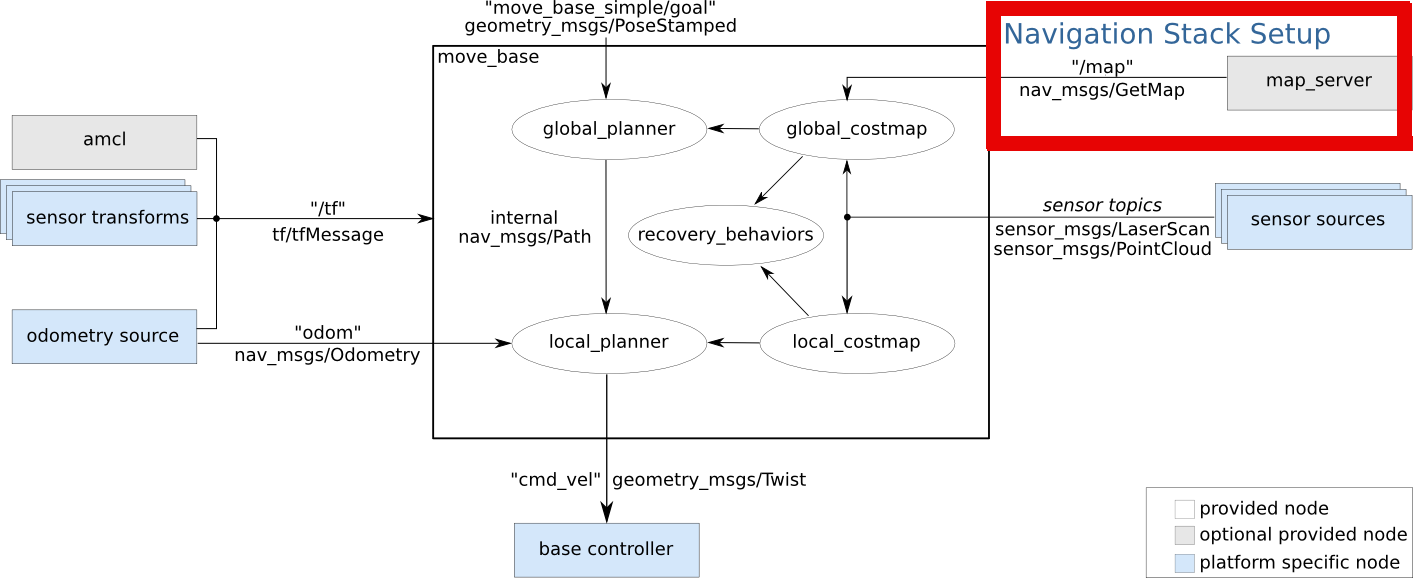
\includegraphics[width=16cm]{img/cap5/navigationstackzoom}
  \end{center}
  \caption{Encuadre de nuestro sistema dentro del modelo de navegación de ROS}
  \label{fig:navigationstackzoom}
\end{figure}

El sistema de mapeado propuesto consta de 3 nodos principales:

\begin{enumerate}
\item Map\_server: Este nodo se encarga de cargar desde fichero el mapa estático y el mapa de largo plazo y activa un servicio para que cualquier otro nodo pueda pedir estos mapas. 
\item Obs\_detector: La función principal de este nodo es la de detectar objetos, leyendo la información proporcionada por el láser, y componer con dicha información el mapa de corto plazo. Para ello solicita los Metadatos de los mapas cargados al nodo Map\_server, creando así un mapa de las mismas medidas y misma resolución que los mapas que maneja el map\_server. Este mapa es publicado para que sea utilizado por el nodo Map\_controller o sea visualizado por la herramienta Rviz.
\item Map\_controller: Nodo que se encarga de la composición del mapa final y de actualizar el mapa de largo plazo con la información obtenida del mapa de corto plazo. Estos mapas son también publicados en distintos topics para que sean utilizados por los nodos encargados de la navegación.
\end{enumerate}
\begin{figure} [H]
  \begin{center}
    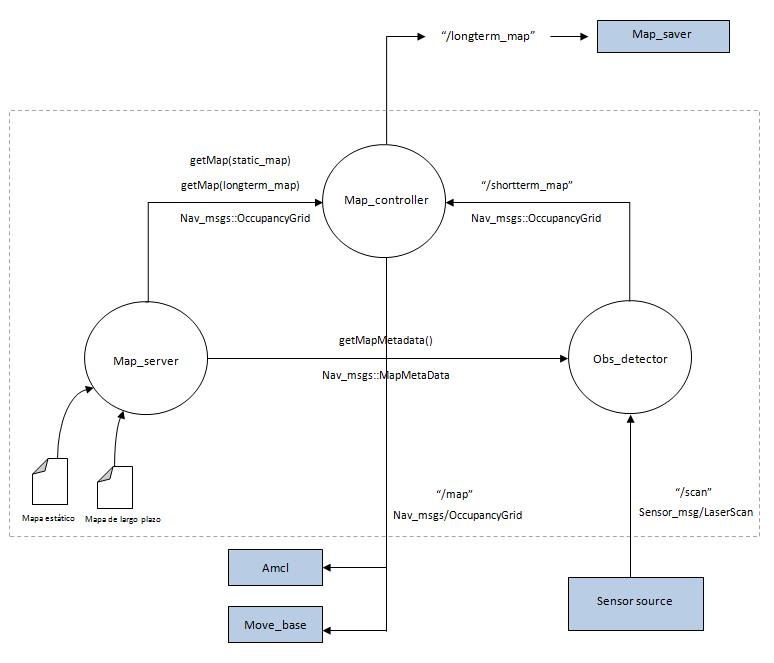
\includegraphics[width=16cm]{img/cap5/esquemaSistema}
  \end{center}
  \caption{Esquema del sistema}
  \label{fig:esquemaSistema}
\end{figure}

\section{Servidor de mapas dinámico}
\label{cap:sevidordemapasdinamico}

En esta sección se describirá el proceso de construcción de los distintos mapas que el servidor de mapas dinámico ofrece, mapa estático, mapa de largo plazo y mapa de corto plazo, así como el proceso de combinación entre ellos para dar lugar al mapa final que será usado por componentes de ROS vistos anteriormente.

\subsection{Mapa estático}
El mapa estático se caracteriza por incluir las partes inmutables del escenario, como son las paredes o las puertas. La mejor manera de construirlo es medir todo el escenario y crear el mapa usando una herramienta de diseño gráfico. En este caso se ha usado \textit{Gimp}.
Este mapa nos servirá como base para crear el mapa de largo plazo.

\begin{figure} [H]
  \begin{center}
    \includegraphics[width=7cm]{img/cap5/mapaestatico}
  \end{center}
  \caption{Mapa estático}
  \label{fig:mapaestatico}
\end{figure}

\subsection{Mapa de corto plazo}
El mapa de corto plazo se caracteriza por ser un mapa en el que se representa los objetos que el robot va percibiendo. Este mapa se inicializa con el valor 255, lo que indica una incertidumbre total. En el instante en el que el algoritmo de construcción del mapa comienza a iterar comenzarán a corregirse estos valores iniciales, asignando el valor 0 a las celdas que corresponden con zonas libres e incrementando desde 0 hasta 254 el valor de las celdas que se perciben como ocupadas.

\renewcommand{\lstlistingname}{Código}
\begin{lstlisting}[caption=Inicialización del cost\_map correspondiente al mapa de corto plazo, label={lst:initcostmap}]

  metadata = getMetadata();
  tf::TransformListener tf(ros::Duration(10));
  cells_size_x = metadata.width;
  cells_size_y = metadata.height;
  resolution = metadata.resolution;
  origin_x = metadata.origin.position.x;
  origin_y = metadata.origin.position.y;
  default_value = 255;
  scan_ready = false;
  pos_ready = false;
  cost_map.resizeMap(cells_size_x,cells_size_y, resolution, origin_x, origin_y);
  cost_map.setDefaultValue(default_value);
  cost_map.resetMap(0,0,cost_map.getSizeInCellsX(), cost_map.getSizeInCellsY());
\end{lstlisting}


El algoritmo propuesto destaca por la capacidad de, no solo añadir objetos al mapa, si no ademas eliminarlos si los objetos desaparecen del lugar que ocupaban. Esto con las herramientas de ROS no puede conseguirse, ya que si solo utilizamos el nodo map\_server para publicar nuestro mapa, tanto el algoritmo de navegación como el de localización cogerán ese mapa y calcularán sobre el nuestra localización y las rutas al destino, pero ese mapa no tendrá en cuenta cambios en el entorno como puede ser una persona paseando por la casa o un mueble cambiado de sitio, es un mapa estático, por lo que puede resultar totalmente erróneo. Por otro lado si usamos la herramienta gmapping para crear nuestro mapa y localizarnos simultáneamente en él, tenemos el mismo problema. En un entorno dinámico con personas moviéndose u objetos cambiando de sitio, se generará un mapa con muchísimo ruido en las zonas libres y con objetos que se mantienen en su lugar cuando ya no están, por lo que la localización empezará a fallar, ya que las muestras del láser no corresponderán con el mapa. 

La solución a este problema se resuelve con la creación de un algoritmo que pueda borrar elementos del mapa. Para ello se compara cada muestra de datos con el mapa que estamos generando y si en dicha muestra existen celdas libres que en el mapa están ocupadas se decrementa el valor de dicha celda en el mapa. La figura \ref{fig:lecturalaser} representa un modelo de una muestra del láser en el que podemos observar lo descrito anteriormente, celdas que marcaremos como ocupadas y celdas que marcaremos como libres. También observamos el límite del láser, que se sitúa en 2.5 metros, a las celdas de mas allá del límite no se les modificará su valor.
La cuantía del decremento se puede modelar, consiguiendo así que el robot olvide más lentamente o más rápidamente los objetos que desaparecen del escenario.

\begin{figure} [H]
  \begin{center}
    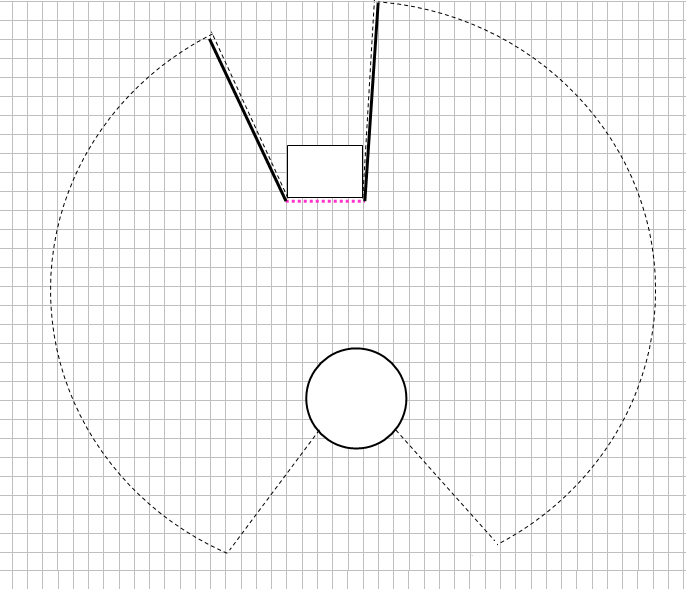
\includegraphics[width=10cm]{img/cap5/lecturaLaser}
  \end{center}
  \caption{Esquematización de una lectura de láser con un objeto.}
  \label{fig:lecturalaser}
\end{figure}


\renewcommand{\lstlistingname}{Código}
\begin{lstlisting}[caption=Función que actualiza el mapa en cada iteración, label={lst:updatecostmap}]
  void
  ObstacleDetector::updateCostmap(){
    if(scan_ready && pos_ready){
      incrementCostProcedure();
      decrementCostProcedure();
    }
    pVectorList_.clear();
    pointList_.clear();
  }
\end{lstlisting}

El proceso de añadir o eliminar un objeto puede ser más o menos rápido dependiendo de los valores de las variables que modelan estas operaciones. Para el caso de nuestro algoritmo contamos un fichero con extensión yaml en el que modificamos los valores de los parámetros.
\renewcommand{\lstlistingname}{Código}
\begin{lstlisting}[caption=Fichero de configuración obstacle\_detector.yaml, label={lst:obstacledetectorconfig}]
  cost_inc: 4
  cost_dec: 1
  min_lenght: 0.23
  max_lenght: 2.5
\end{lstlisting}
Los valores asociados a cost\_inc y cost\_dec representan el incremento o decremento del valor de una celda por cada iteración del algoritmo. Los otros valores configurables representan la longitud máxima y mínima que se tiene en cuenta para cada medida que el láser nos proporciona.

Al final de cada iteración del algoritmo el mapa de corto plazo es publicado en un topic para que pueda ser usado por el resto de nodos que conforman el servidor de mapas dinámico. Para llevar a cabo esta operación usamos una estructura de datos proporcionada por ROS, \textit{Costmap2DPublisher}\footnote{http://docs.ros.org/indigo/api/costmap\_2d/html/classcostmap\_\_2d\_1\_1Costmap2DPublisher.html}. Este publicador publica nuestro mapa en el topic \textit{/shortterm\_map}.


\renewcommand{\lstlistingname}{Código}
\begin{lstlisting}[caption=Step del nodo obstacle\_detector, label={lst:stepobstacledetector}]
  void
  ObstacleDetector::step(){
    updateCostmap();
    cost_map_publisher_.publishCostmap();
  }

  int
  main(int argc, char** argv)
  {
    ros::init(argc, argv, "obstacle_detector");   //Inicializa el nodo
    ObstacleDetector obs;
    ros::Rate loop_rate(5);

    while (ros::ok()){
      obs.step();
      ros::spinOnce();
      loop_rate.sleep();
    }
    return 0;
  }

\end{lstlisting}

Existe un pequeño cambio en los valores del mapa que se publica. El tipo de mensaje que se usa para publicar un costmap es \textit{nav\_msgs::OccupancyGrid}\footnote{http://docs.ros.org/indigo/api/nav\_msgs/html/msg/OccupancyGrid.html}. Este tipo de mensaje contiene, ademas de los metadatos asociados al mapa, un array de datos que representa al mapa. La principal diferencia con un costmap es que los valores en un OccupancyGrid van de 0 a 100 y -1 para las celdas desconocidas ,y no de 0 a 255 como en un costmap.

\subsection{Mapa de largo plazo}
El mapa de largo plazo se inicializa con los valores del mapa estático y se caracteriza por incluir los objetos que tienen un valor muy alto en el mapa de corto plazo, por tanto tenemos un mapa con objetos que han perdurado en el mapa a corto plazo durante un largo periodo de tiempo y que podemos considerar que nos van a influir a la hora de planificar nuestra ruta por el escenario. 
Este mapa también es dinámico, por lo que también elimina los objetos del mapa si estos desaparecen o cambian su posición.


\begin{lstlisting}[caption=Procedimiento para añadir un objeto al mapa de largo plazo, label={lst:addobjectlongmap}]
  void
  MapController::updateLongTermMap(nav_msgs::OccupancyGrid s_map){
    for(int i = 0;i<s_map.data.size();i++){
      if(s_map.data[i] > 95){
        longTerm_map.data[i] = s_map.data[i]; 
        .
        .
        .
      }
    }
  }


\end{lstlisting}

En el código mostrado en \ref{lst:addobjectlongmap} muestra el proceso de adición de un objeto al mapa de largo plazo. Para ello se recorren los valores del mapa de corto plazo y si alguno tiene un valor mayor a 95, valor que consideramos lo suficientemente alto como para que sea muy fiable que esa celda está ocupada, se incluye con ese valor al mapa.

\begin{lstlisting}[caption=Procedimiento para eliminar un objeto al mapa de largo plazo, label={lst:deleteobjectlongmap}]
  void
  MapController::updateLongTermMap(nav_msgs::OccupancyGrid s_map){
    for(int i = 0;i<s_map.data.size();i++){
      .
      .
      .
      }else if(s_map.data[i] < 5 && s_map.data[i] >= 0 && longTerm_map.data[i] >= longterm_cost_dec && static_map.data[i] < 95){
        longTerm_map.data[i] = longTerm_map.data[i] - longterm_cost_dec;
      }
    }
  } 

\end{lstlisting}

En el código mostrado en \ref{lst:deleteobjectlongmap} se compara el mapa de largo plazo con el mapa de corto plazo. Si una celda en el mapa de largo plazo tiene un valor que indica que está ocupada y en el mapa de corto plazo esa misma celda tiene un valor que indica que está libre, siempre y cuando esa celda no pertenezca a una celda de una pared, se decrementa su valor en el mapa de largo plazo. La cuantía de este decremento también puede modelarse, longterm\_cost\_dec, regulando así la memoria que tenemos de los objetos que hemos añadido a este mapa.\pagebreak

Por último publicamos el mapa en el topic \textit{/longTerm\_map}.

\begin{lstlisting}[caption=Publicación del mapa de largo plazo, label={lst:longmappublish}]
longTermMap_pub   = nh_.advertise<nav_msgs::OccupancyGrid>("/longTerm_map", 5); 

void
MapController::publishAll(){
  .
  .
  .
  longTerm_map.header.stamp = ros::Time::now();
  longTermMap_pub.publish(longTerm_map);
}
\end{lstlisting}

Adicionalmente este mapa se guarda cada cierto tiempo en un fichero, usando el nodo por defecto de ROS para este fin ,\textit{map\_saver}\footnote{http://wiki.ros.org/action/fullsearch/map\_server\#map\_saver}. Así por ejemplo podemos tener un cuenta una mesa dentro del salón de una casa para una futura ejecución del algoritmo. Esto nos permitiría planificar una ruta mejor para la navegación, ya que podríamos esquivar esta mesa con facilidad y llegar a nuestro destino lo más rápido posible. Si no tuviéramos esta mesa en cuenta el algoritmo podría planificar una ruta a través de las celdas ocupadas por la mesa. Seguramente el robot no llegaría a chocar, ya que el planificador de rutas usa un pequeño mapa local para evitar estos problemas, pero es seguro que tardaría más en alcanzar su destino ya que al encontrarse frente a la mesa el robot se pararía y tendría que recalcular una nueva ruta. 

\section{Construcción del mapa final}
\label{sec:construccionmap}
El mapa final será la composición de los mapas de largo plazo, que ya incluye el mapa estático, y de corto plazo. Este mapa será usado por el nodo de la navegación y por el nodo de la localización para navegar y localizar al robot en el escenario. La composición del mapa final o mapa efectivo será el resultado de la operación de máximo entre los mapas de corto y de largo plazo, como vemos en el código del apartado \ref{lst:buildEffectivemap}. De esta manera incluiremos en el mapa final toda la información relacionada con los objetos que llevan un tiempo en la escena y también incluiremos, aunque con un menor valor, personas o cosas que acaban de entrar en las inmediaciones del robot.
\endinput
\pagebreak

\begin{lstlisting}[caption=Composición del mapa final, label={lst:buildEffectivemap}]
  void
  MapController::buildEffectiveMap(nav_msgs::OccupancyGrid s_map,nav_msgs::OccupancyGrid l_map){
    for(int i = 0;i<s_map.data.size();i++){
      effective_map.data[i] = std::max(s_map.data[i],l_map.data[i]);
    }
  }
\end{lstlisting}


Tras la creación del mapa este es publicado en el topic \textit{/map}. 

\begin{lstlisting}[caption=Publicación del mapa final, label={lst:effectivemappublish}]
effectiveMap_pub = nh_.advertise<nav_msgs::OccupancyGrid>("/map", 5);

void
MapController::publishAll(){
  effective_map.header.stamp = ros::Time::now();
  effectiveMap_pub.publish(effective_map);
  .
  .
  .
}
\end{lstlisting}


\subsubsection{Mapeado de zonas desconocidas}
\label{sec:mapeadozonadesconocida}
La creación de un mapa de corto plazo a partir de las muestras del láser y la posterior incorporación del mapa de largo plazo para generar un mapa conjunto cuenta con una gran versatilidad y eficacia, tanto que es posible mapear nuevas zonas o estancias del escenario. Generar un mapa así nos permite también localizarnos en este e incluso navegar por el. 

No contamos con un sistema de SLAM, ya que partimos de unos mapas, pero poder incluir en un mapa objetos o nuevas estancias nos permite mantener nuestro robot doméstico por mucho más tiempo navegando por nuestra casa, lo que lo hace mucho más robusto y versátil. Esta ventaja podría, por ejemplo, aplicarse a un robot sirviente en una universidad. Al principio, como prueba de la tecnología, puede que nos interese darle una pequeña zona mapeada por la que moverse, pero si un día queremos que su rango de efectividad se amplíe solo tendremos que moverlo por la zona deseada y se añadirá al mapa perfectamente.



% Capitulo 6
\chapter{Experimentación}
\label{cap:experimentacion}

\section {Mapeado en entorno doméstico}
\label{cap:mapeadodomestico}

\section {Navegación con obstáculos dinámicos}
\label{cap:navegacionconobstaculos}

\section {Experimentación en la Robocup}
\label{cap:experimentacionrobocup}



{Navegacion por entornos desconocidos}

Además esta modificación nos ha permitido localizarnos en entornos desconocidos, es decir, ahora contamos con la capacidad de navegar por estancias de una casa que no tenemos en el mapa. Estas estancias se irán añadiendo al mapa de corto plazo primero y más tarde al mapa de largo plazo y el algoritmo de localización puede seguir calculando nuestra posición en los nuevos mapas.

\begin{figure}[hbtp]
  \begin{center}
    \includegraphics[width=12cm,height=7cm]{img/cap6/grannieAnne-ext}
  \end{center}
  \caption{Escenario extendido}
  \label{fig:grannieAnne-ext}
\end{figure}

\begin{figure}[hbtp]
  \begin{center}
    \includegraphics[width=10cm,height=6cm]{img/cap6/localization-ext}
  \end{center}
  \caption{Detalle de la localización}
  \label{fig:localization-ext}
\end{figure}


\begin{figure}[hbtp]
  \begin{center}
    \subfigure[Mapa total]{\includegraphics[width=12cm,height=7cm]{img/cap6/map-ext}}
    \subfigure[Mapa de largo plazo]{\includegraphics[width=12cm,height=7cm]{img/cap6/longmap-ext}}
    \subfigure[Mapa de corto plazo]{\includegraphics[width=12cm,height=7cm]{img/cap6/shortmap-ext}}
  \end{center}
  \caption{Mapas del escenario extendido}
  \label{fig:maps-ext}
\end{figure}

En la figura \ref{fig:grannieAnne-ext} vemos como el escenario ha sido extendido, añadiéndole unos pasillos a la derecha de la casa. El mapa estático usado es el mismo que el mostrado en la figura \ref{fig:mapaestatico}. Vemos como después de recorrer la parte desconocida del mapa se ha añadido al mapa de largo plazo y también al mapa total, figura \ref{fig:maps-ext}. Observamos en las flechas rojas bajo el robot que la incertidumbre en la posición del robot es mínima, figura \ref{fig:localization-ext}. 

% Capitulo 7
\chapter{Experimentación}
\label{cap:experimentacion}
En este capitulo desarrollaremos e ilustraremos los diferentes experimentos o pruebas unitarias que se han realizado para la validación del sistema de mapeado dinámico y el sistema de navegación semántica. En primer lugar se realizarán test de mapeado en un entorno doméstico. Con esto comprobaremos que los objetos son eliminados del mapa si desaparecen y como el mapa va cambiando. También haremos pruebas en una estancia de la casa que no aparece en los mapas y comprobaremos como se añade correctamente al mapa. En segundo lugar haremos pruebas de navegación en un entorno doméstico y dinámico y por ultimo expondremos los experimentos llevados a cabo en la RoboCup@Home en el transcurso de la competición.

\section {Mapeado en entorno doméstico}
\label{cap:mapeadodomestico}
En esta primera sección se expondrán los experimentos realizados para validar el proceso por el cual se incluyen o se eliminan los objetos del primer mapa que maneja el servidor de mapas dinámico, el mapa de corto plazo. Estos experimentos se realizarán primero en el simulador Gazebo con el mapa GrannieAnnie, y después en el robot real en el laboratorio.

\subsection {Adición y eliminación de objetos en el mapa de corto plazo en entorno simulado}
\label{sec:add-deleteobjects}

La figura \ref{fig:initserver} fue captada al iniciar el algoritmo. Observamos que la mayor parte del mapa de corto plazo se encuentra en una posición de desconocimiento y que se han ido incluyendo en este las zonas libres, las paredes y la estantería. Los puntos morados y verdes corresponden a la representación de las muestras tomadas por el láser.

\begin{figure}[hbtp]
  \begin{center}
    \subfigure[]{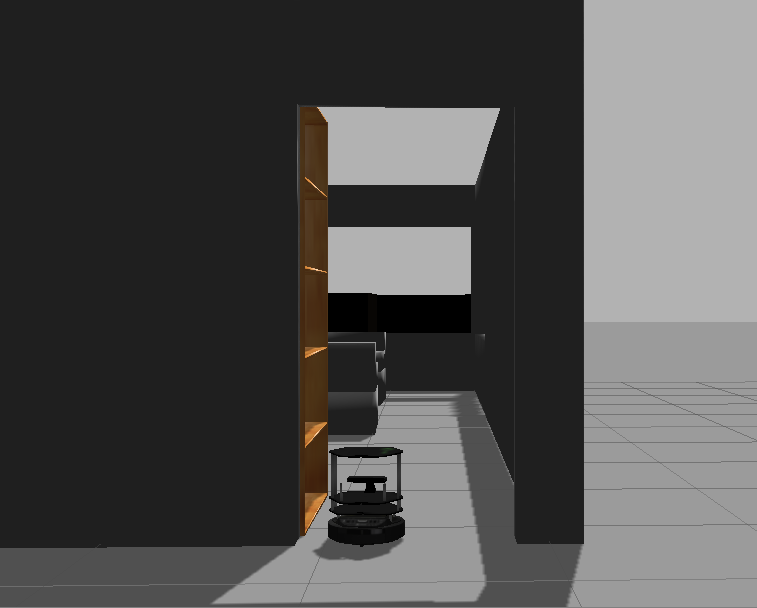
\includegraphics[width=5cm,height=5cm]{img/cap7/incrementmap}}
    \subfigure[]{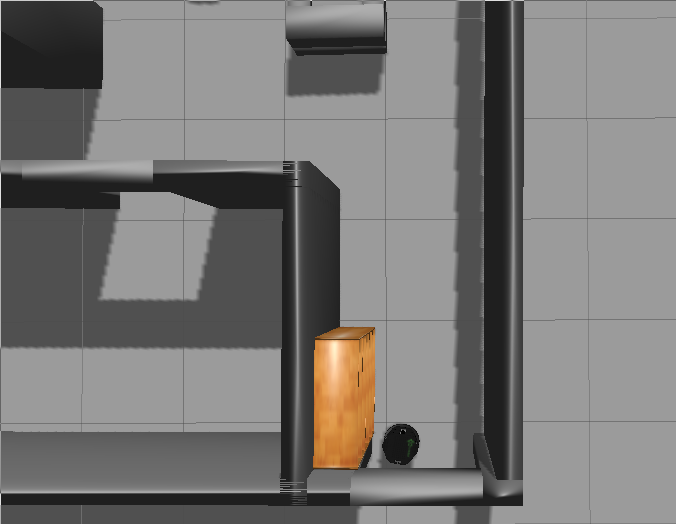
\includegraphics[width=5cm,height=5cm]{img/cap7/incrementmap2}}
    \subfigure[]{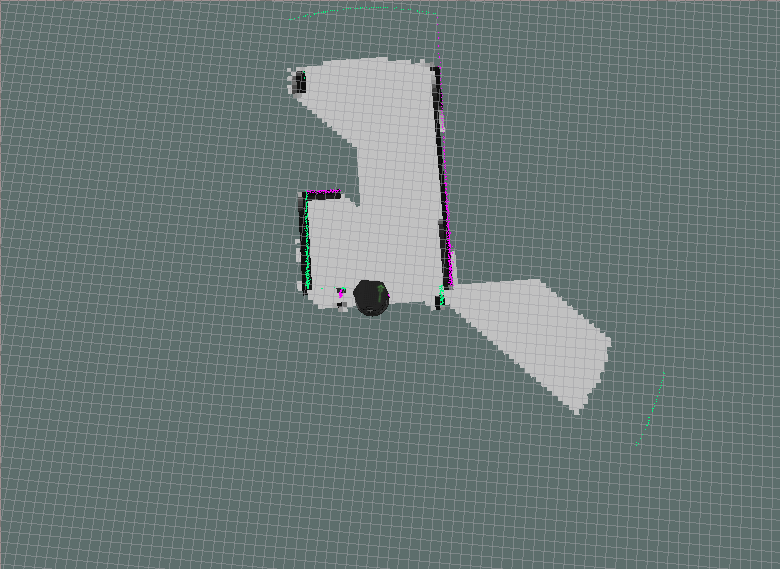
\includegraphics[width=5cm,height=5cm]{img/cap7/incrementmap-rviz}}
  \end{center}
  \caption{Visión del simulador, (a) y (b), y mapa a corto plazo (c).}
  \label{fig:initserver}
\end{figure}

Tras el inicio del algoritmo se añadió un objeto nuevo al escenario. Esto se representa en la figura \ref{fig:includeobject}. Vemos como el objeto ha sido reconocido por el láser, ya que podemos observar su contorno en las marcas de colores verdes y que el algoritmo añade el objeto al mapa y lo sitúa en una posición coherente respecto a la posición que ocupa el objeto en el escenario simulado.

\begin{figure} [hbtp]
  \begin{center}
    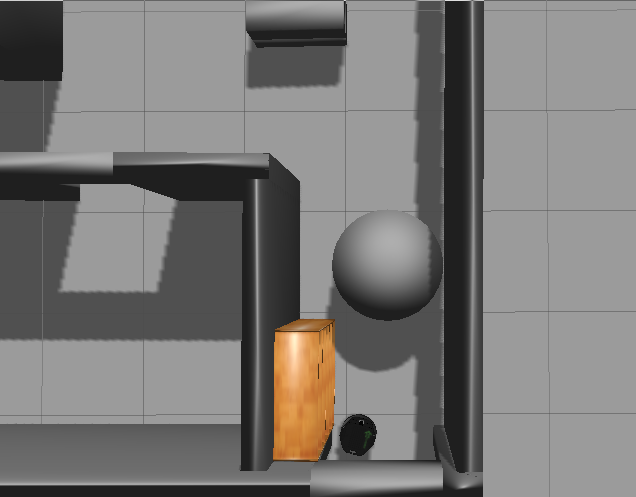
\includegraphics[width=6cm,height=5cm]{img/cap7/incrementmap-object3}
    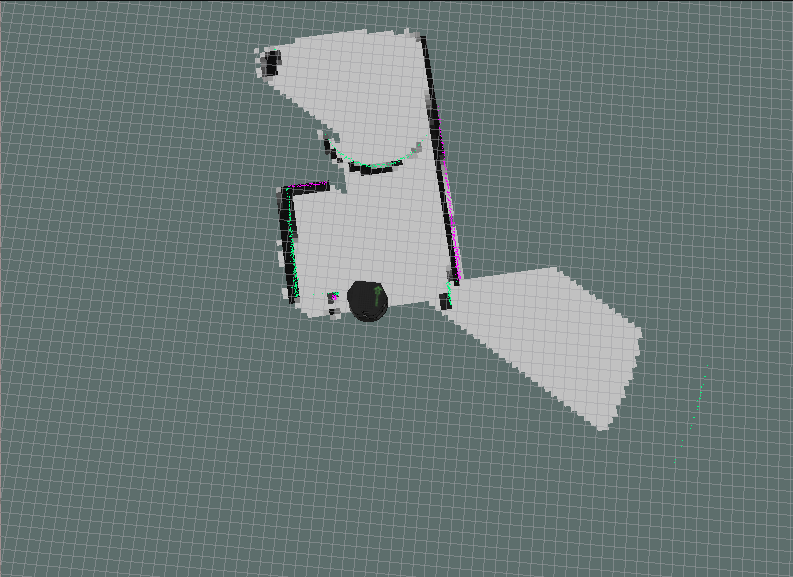
\includegraphics[width=6cm,height=5cm]{img/cap7/incrementmap-object}
  \end{center}
  \caption{Añadimos un objeto al escenario}
  \label{fig:includeobject}
\end{figure}

Una vez que el algoritmo a incluido el objeto en el mapa procedemos a eliminarlo del escenario simulado. Se observa también que las marcas del láser ya no aparecen superpuestas en el mapa. Esto se representa en la figura  \ref{fig:deleteobject}. Vemos como el algoritmo ha comenzado a borrar el objeto, por lo que el valor de las celdas que estaban ocupadas por el objeto ahora es mucho menor.

\begin{figure}[hbtp]
  \begin{center}
    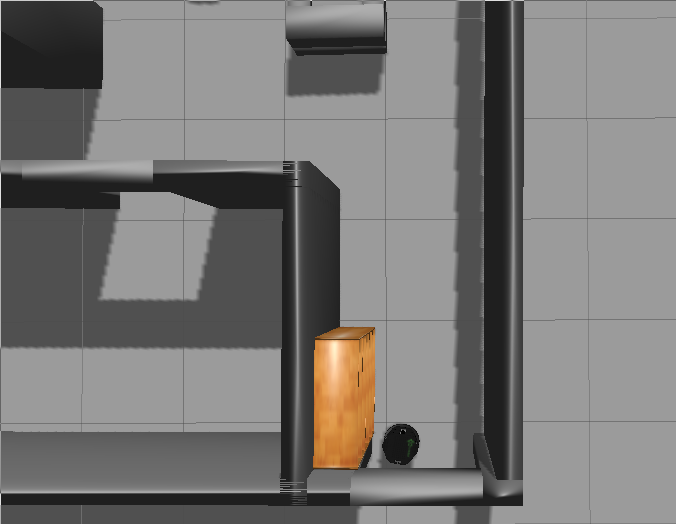
\includegraphics[width=6cm,height=5cm]{img/cap7/incrementmap2}
    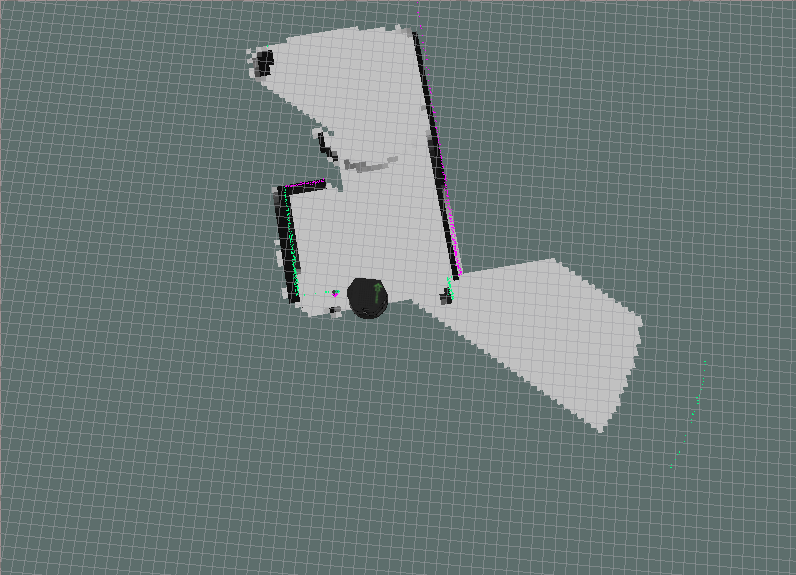
\includegraphics[width=6cm,height=5cm]{img/cap7/incrementmap-object2}
  \end{center}
  \caption{Eliminamos un objeto del escenario}
  \label{fig:deleteobject}
\end{figure}

\subsection {Adición y eliminación de objetos en el mapa de corto plazo en entorno real}
\label{sec:add-deleteobjectsreal}

GRAFICA ADICION: RELACION VALOR VARIABLE / TIEMPO
GRAFICA BORRADO: RELACION VALOR VARIABLE / TIEMPO

\subsection {Adición y eliminación de objetos en el mapa de largo plazo en entorno simulado}
\label{sec:add-deleteobjectslong}
En el siguiente experimento probaremos el añadido y borrado de objetos en el mapa de largo plazo. Para ello realizamos el mismo experimento que en la sección anterior aunque ahora el objeto en el camino del robot es un sofá. Observamos en la figura \ref{fig:addobjectlongmap} como se encuentra el nuevo objeto y al cabo de un tiempo lo añade al mapa de largo plazo. 
\begin{figure}[hbtp]
  \begin{center}
    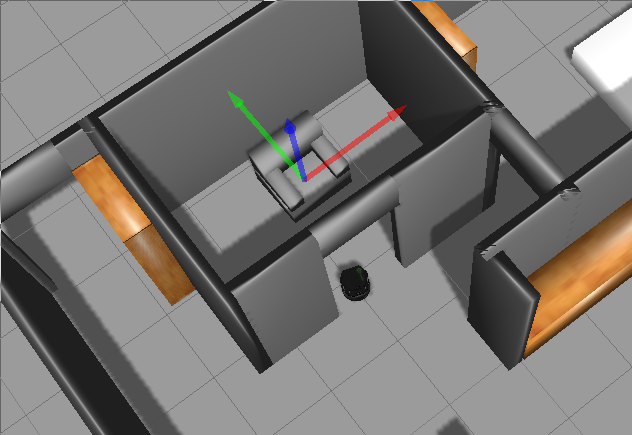
\includegraphics[width=10cm,height=6cm]{img/cap7/addingobject-gazebo}
    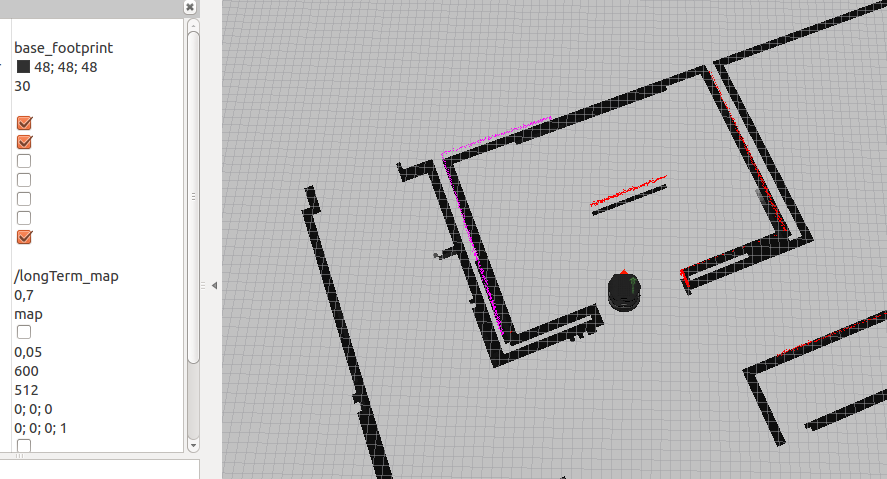
\includegraphics[width=10cm,height=5cm]{img/cap7/addingobject-longmap}
  \end{center}
  \caption{Añadimos un objeto al mapa de largo plazo}
  \label{fig:addobjectlongmap}
\end{figure}
En la figura \ref{fig:deleteobjectlongmap} el objeto ha sido eliminado del entorno simulado y el algoritmo comienza a borrarlo también del mapa de largo plazo. Observamos como ha disminuido el valor de las celdas ocupadas anteriormente por el sofá.

\begin{figure}[hbtp]
  \begin{center}
    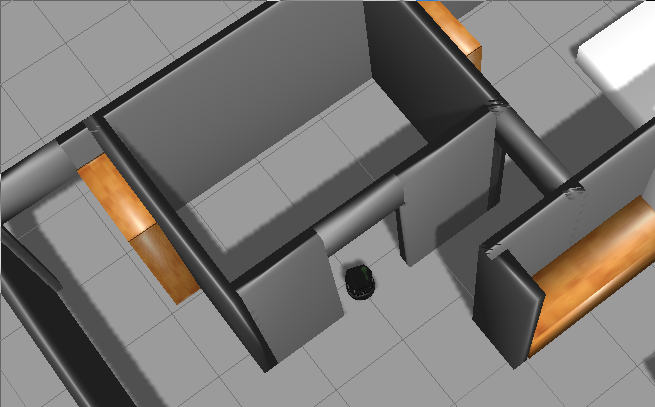
\includegraphics[width=10cm,height=5cm]{img/cap7/deletingobject-gazebo}
    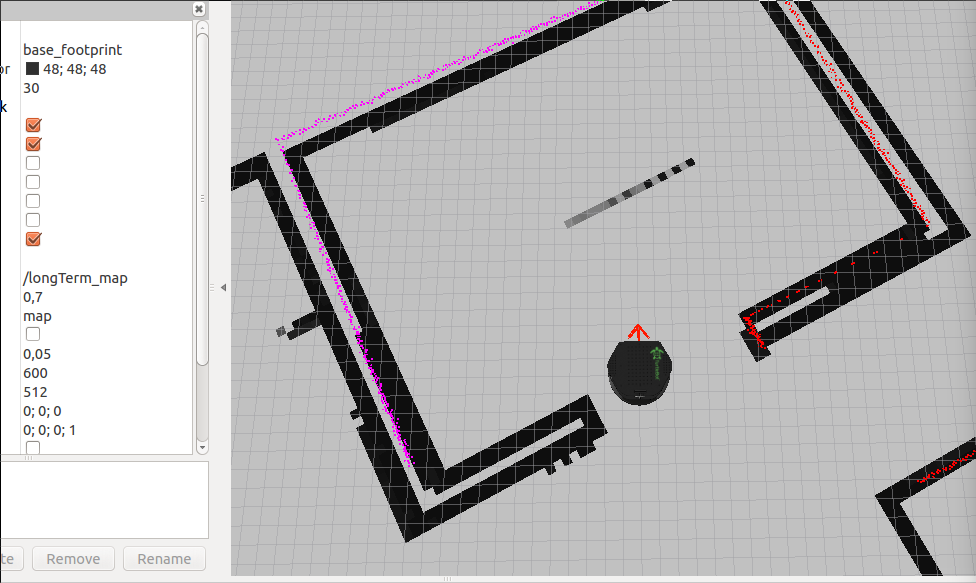
\includegraphics[width=10cm,height=5cm]{img/cap7/deletingobject-longmap}
  \end{center}
  \caption{Borramos un objeto del mapa de largo plazo}
  \label{fig:deleteobjectlongmap}
\end{figure}

GRAFICA BORRADO: RELACION VALOR VARIABLE / TIEMPO

\subsection {Mapeado de zonas desconocidas.}
Para este experimento se ha extendido ligeramente el mapa simulado, de tal forma que se han añadido unos pasillos nuevos a la derecha del escenario, como vemos en la figura \ref{fig:grannieAnne-ext}. Esta zona no vamos a incluirla previamente en el mapa estático ni en el mapa de largo plazo y queremos comprobar si el sistema es capaz de añadir una zona nueva al mapa y localizarse correctamente. El mapa estático usado es el mismo que el mostrado en la figura \ref{fig:mapaestatico}.
\begin{figure}[H]
  \begin{center}
    \includegraphics[width=12cm,height=7cm]{img/cap7/grannieAnne-ext}
  \end{center}
  \caption{Escenario extendido}
  \label{fig:grannieAnne-ext}
\end{figure}

\begin{figure}[hbtp]
  \begin{center}
    \includegraphics[width=10cm,height=6cm]{img/cap7/localization-ext}
  \end{center}
  \caption{Detalle de la localización}
  \label{fig:localization-ext}
\end{figure}

\begin{figure}[hbtp]
  \begin{center}
    \subfigure[Mapa total]{\includegraphics[width=12cm,height=7cm]{img/cap7/map-ext}}
    \subfigure[Mapa de largo plazo]{\includegraphics[width=12cm,height=7cm]{img/cap7/longmap-ext}}
    \subfigure[Mapa de corto plazo]{\includegraphics[width=12cm,height=7cm]{img/cap7/shortmap-ext}}
  \end{center}
  \caption{Mapas del escenario extendido}
  \label{fig:maps-ext}
\end{figure}

  Vemos como después de recorrer la parte desconocida del mapa se ha añadido al mapa de largo plazo y también al mapa total, figura \ref{fig:maps-ext}. Observamos en las flechas rojas bajo el robot que la incertidumbre en la posición del robot es mínima, figura \ref{fig:localization-ext}. Comprobamos con este experimento la potencia de esta característica de nuestro sistema, somos capaces de añadir zonas completas al mapa sin necesidad de reiniciar el algoritmo ni de modificar el mapa estático, y seguir completamente localizados.

\subsection {Adición y eliminación de objetos en el mapa de largo plazo en entorno real}
\label{sec:add-deleteobjectslongreal}

\section {Navegación con obstáculos dinámicos}
\label{cap:navegacionconobstaculos}

\section {Experimentación en la Robocup}
\label{cap:experimentacionrobocup}

El día 27 de Junio de 2016 el equipo Gentlebot viajó a Leipzig para participar en la Robocup 2016, en la categoría Home. El equipo lo formábamos 4 personas de la universidad de León y 4 personas de la URJC. En este apartado detallaremos las distintas actividades llevadas a cabo en los días de preparación y en los días de competición. 

El robot con el que participamos en la competición, detallado en el capitulo XXX, fue el RB1. Las pruebas a disputar fueron las siguientes: Navigation, Speech Recognition \& Audio Detection, Person Recognition, Manipulation \& Object Recognition, Following \& Guiding y General Purpose Service Robot y estas pruebas se disputarían en 2 escenarios desconocidos a priori, tanto en dimensiones como en los objetos que contendrían. El sistema de navegación propuesto estaba involucrado en las pruebas de Navigation, Following \& Guiding y General Purpose Service Robot. 

\begin{itemize}
\item \textbf{Día 1.} Una vez nos instalamos y montamos el robot, que para el viaje hubo que desmontar algunas partes, nos dispusimos a medir las dos arenas para crear los mapas estáticos. Los equipos estábamos organizados en turnos para usar los escenarios y así probar los mapas o anotar \textit{waypoints} por los que el robot debiera pasar o alcanzar. Una vez creados los mapas estáticos y hacer que el robot creara los mapas de largo plazo con algunos objetos que había en las arenas, nos dispusimos a retocarlos ligeramente. Al no disponer del robot RB1 físicamente hasta la llegada a la competición no tuvimos en cuenta algunos detalles, como por ejemplo que el robot no podía pasar por debajo de una mesa por ser mucho más alto que el robot kobuki. Esto no tendría por qué haber sido un impedimento, pero los árbitros de la competición situaron mesas muy cercanas a las puertas por las que el robot tendría que entrar en la arena. Esto generaba que la ruta que establecía el nodo \textit{move\_base} cruzaba la mesa y ademas el robot, al tener el láser en la base, no añadía al mapa un objeto de las dimensiones de una mesa, solo añadía las patas. Por esto hubo que añadir a mano algunos objetos al mapa de largo plazo. Tras esto también empezamos a preparar y a ensayar la prueba de Inspección que tienen que pasar todos los robots que tendría lugar al día siguiente.
\item \textbf{Día 2.} En el día 2 se anunció en que arena tendría lugar la inspección y en por qué puerta se entraría a la inspección, por lo que cogimos un punto de referencia en esa puerta para establecerlo como punto de inicio del robot dentro del mapa. También comenzamos a preparar la prueba de navegación que tendría lugar al día siguiente y que involucraba las 2 arenas, ya que se haría en 3 tandas y se iría alternando de arena. La inspección consistía en entrar en la arena y acercarse a un mueble, este era el \textit{waypoint 1}. Entre el mueble y el robot se colocaba un árbitro al que el robot no podía tocar. Una vez el robot comenzaba a sortear al arbitro este se retiraba. Al llegar al \textit{waypoint 2} el robot se paraba y esperaba que un arbitro se enseñara un código QR que el indicaba que debía continuar. Tras esto el robot cruzaba una puerta y si todo estaba correcto los árbitros probaban el botón de emergencia, parando el robot y finalizando así la prueba. El resto del día anotamos los diferentes \textit{waypoints} de la prueba de navegación, ensayamos en las arenas con estos waypoints y preparamos otras pruebas del día 3, como la prueba de Speech Recognition \& Audio Detection.
\item \textbf{Día 3.} El comienzo del día 3 nos deparó una pequeña sorpresa. No sabíamos, o no teníamos del todo claro, si la puerta de la arena iba a estar cerrada o abierta al comenzar la prueba, por lo que no teníamos del todo claro cuando se debía lanzar el algoritmo de navegación. Los jueces nos aclararon que se debía lanzar todos los algoritmos y en ese momento llamar a la puerta y desde dentro un juez nos abriría. Este primer escollo nos costó no puntuar en la primera manga de la prueba de navegación, aunque pudimos solventarlo antes de las siguientes tandas. En la segunda tanda, el robot pasó correctamente por la puerta y comenzó a navegar por la casa, sorteando una mesa primero, a un juez después y cambió de ruta cuando una puerta se cerró cuando estaba a punto de pasar por ella. Una silla de finas patas metálicas arruinó nuestra prueba cuando la pusieron entre el robot y la puerta de la habitación. 

En la tercera tanda nos esperaba el más difícil todavía, sortear un vaso de 5cm de altura, que aunque RB1 pudo recalcular bien su ruta para intentar esquivarlo no pudo evitar tocarlo ligeramente para más tarde volver a toparse con una silla en el camino. 

Las pruebas de Speech Recognition \& Audio Detection salieron muy bien, siendo uno de los equipos que mayor puntuación.

\item \textbf{Día 4.} El cuarto día fue nuestro último día como participantes en la RoboCup@Home ya que no obtuvimos los suficientes puntos para clasificarnos para la siguiente fase. La pruebas en las que participamos en este día fueron: Manipulation \& Object Recognition y Following \& Guiding. En la primera no obtuvimos unos buenos resultados ya que no fuimos capaces de reconocer los objetos que se nos presentaron y en la segunda tampoco, ya que no fuimos capaces de reconocer correctamente al árbitro para después seguirle. Esta prueba hubiera sacado mucho partido a la parte del algoritmo en la que se van añadiendo zonas nuevas al mapa ya que consistía en seguir a un árbitro por fuera de las arenas, una zona no mapeada, y luego devolverle a casa.
\end{itemize}




% Capitulo 8
\chapter{Conclusiones y trabajos futuros}
\label{cap:conclusiones}


Con esta aplicación hacemos un uso intensivo de las herramientas de navegación y localización que nos ofrece ROS e incluimos nuestro servidor de mapas dinámico para aportarle mucha más fiabilidad, estabilidad y una memoria a largo plazo necesaria en este tipo de entornos. Ademas asentamos las bases para una interfaz hombre-maquina con la que se pudiera dirigir a nuestro robot a estancias del hogar abstrayéndonos totalmente de distancias o de celdas, con tan solo un comando de voz o un toque en una pantalla táctil que se tradujera en una de las etiquetas con las que hemos identificado cada habitación.

% Bibliografía
\clearpage
\addcontentsline{toc}{chapter}{Bibliografía}
\nocite{*}	% Imprime todas las cites de la bibliografía aunque no se citen
\bibliographystyle{named} 
\bibliography{bibliografia}

\printindex 

\end{document}
